
\section{Simulations, estimations of counting rates and accidentals}\label{sec:simu}

The estimates of counting rates accidentals have been performed using G4SBS, the GEANT4-based simulation package developed for the SBS experiment \cite{g4sbs}.
This package includes a wide range of event generators, which allows us to evaluate the rates for both events of interest (signal) and background.
%, such as elastic/quasi-elastic.
The representation of the experiment apparatus in G4SBS is shown in the high $\epsilon$ configuration in Fig.~\ref{fig:g4sbssetup}. 

\begin{figure}[!h]
  \centering
    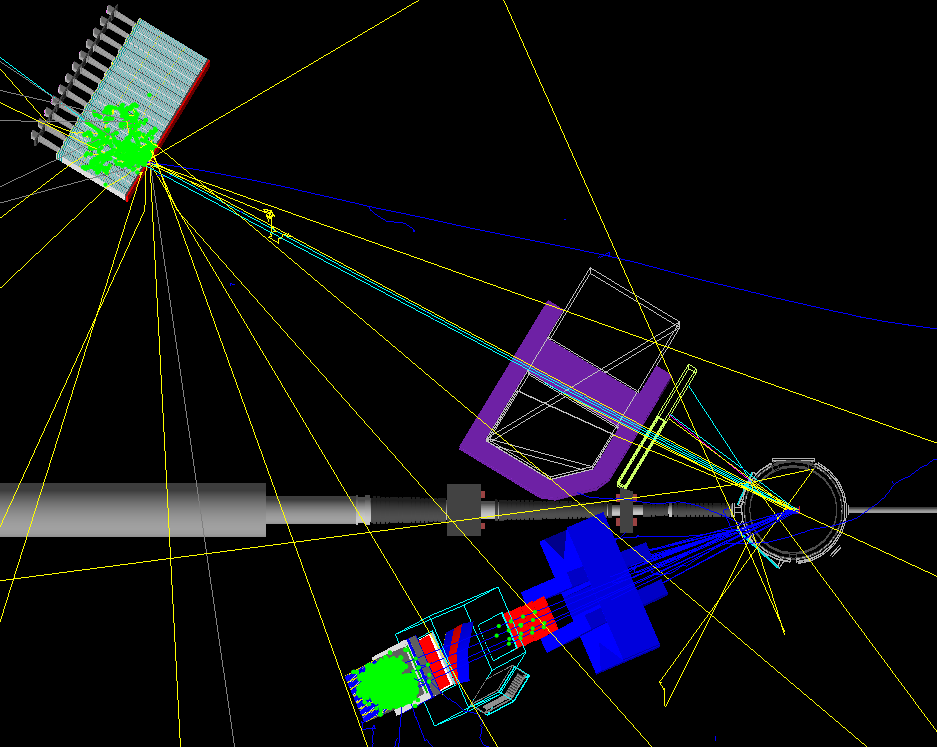
\includegraphics[width=9.6cm,height=8cm]{Plots/SetupHiEPoint.png}
    \caption{Top view of the experimental apparatus model in G4SBS, shown in the high $\epsilon$ configuration. The beam direction is indicated, as well as the main elements (HCal, SBS magnet, BigBite spectrometer)}
    \label{fig:g4sbssetup}
\end{figure}

\subsection{Background and trigger rates}
The main processes expected to contribute to the trigger rates for the BigBite spectrometer are:
%
\begin{itemize}
\item{the inelastic electron nucleon scattering process;}
\item{photons from inclusive $\pi^0$ production;}
\item{and to a lesser extent, charged pions.}
\end{itemize}
%
Concerning HCal, various hadronic backgrounds are expected to contribute to the rates in HCal, the dominant ones being pions.
Both the inelastic scattering and the inclusive neutral and charged pion production are implemented in G4SBS, the latter relying on the Wiser parametrization \cite{wiser}.
The minimum-bias ``beam-on-target'' generator (including all electromagnetic and hadronic processes) has also been considered for the HCal background.

The thresholds to apply to each arm are determined as a function of the elastic peak.
For the electron arm, the threshold has been set at $\mu_E - 2.5 \sigma_E$,  $\mu_E$ and $\sigma_E$ being respectively the position and width of the fitted elastic peak. 
Fig.~\ref{fig:BBRates} presents the distributions of rate of energy deposit for the different processes involved in the BigBite trigger rates. 

\begin{figure}[!h]
  \centering
    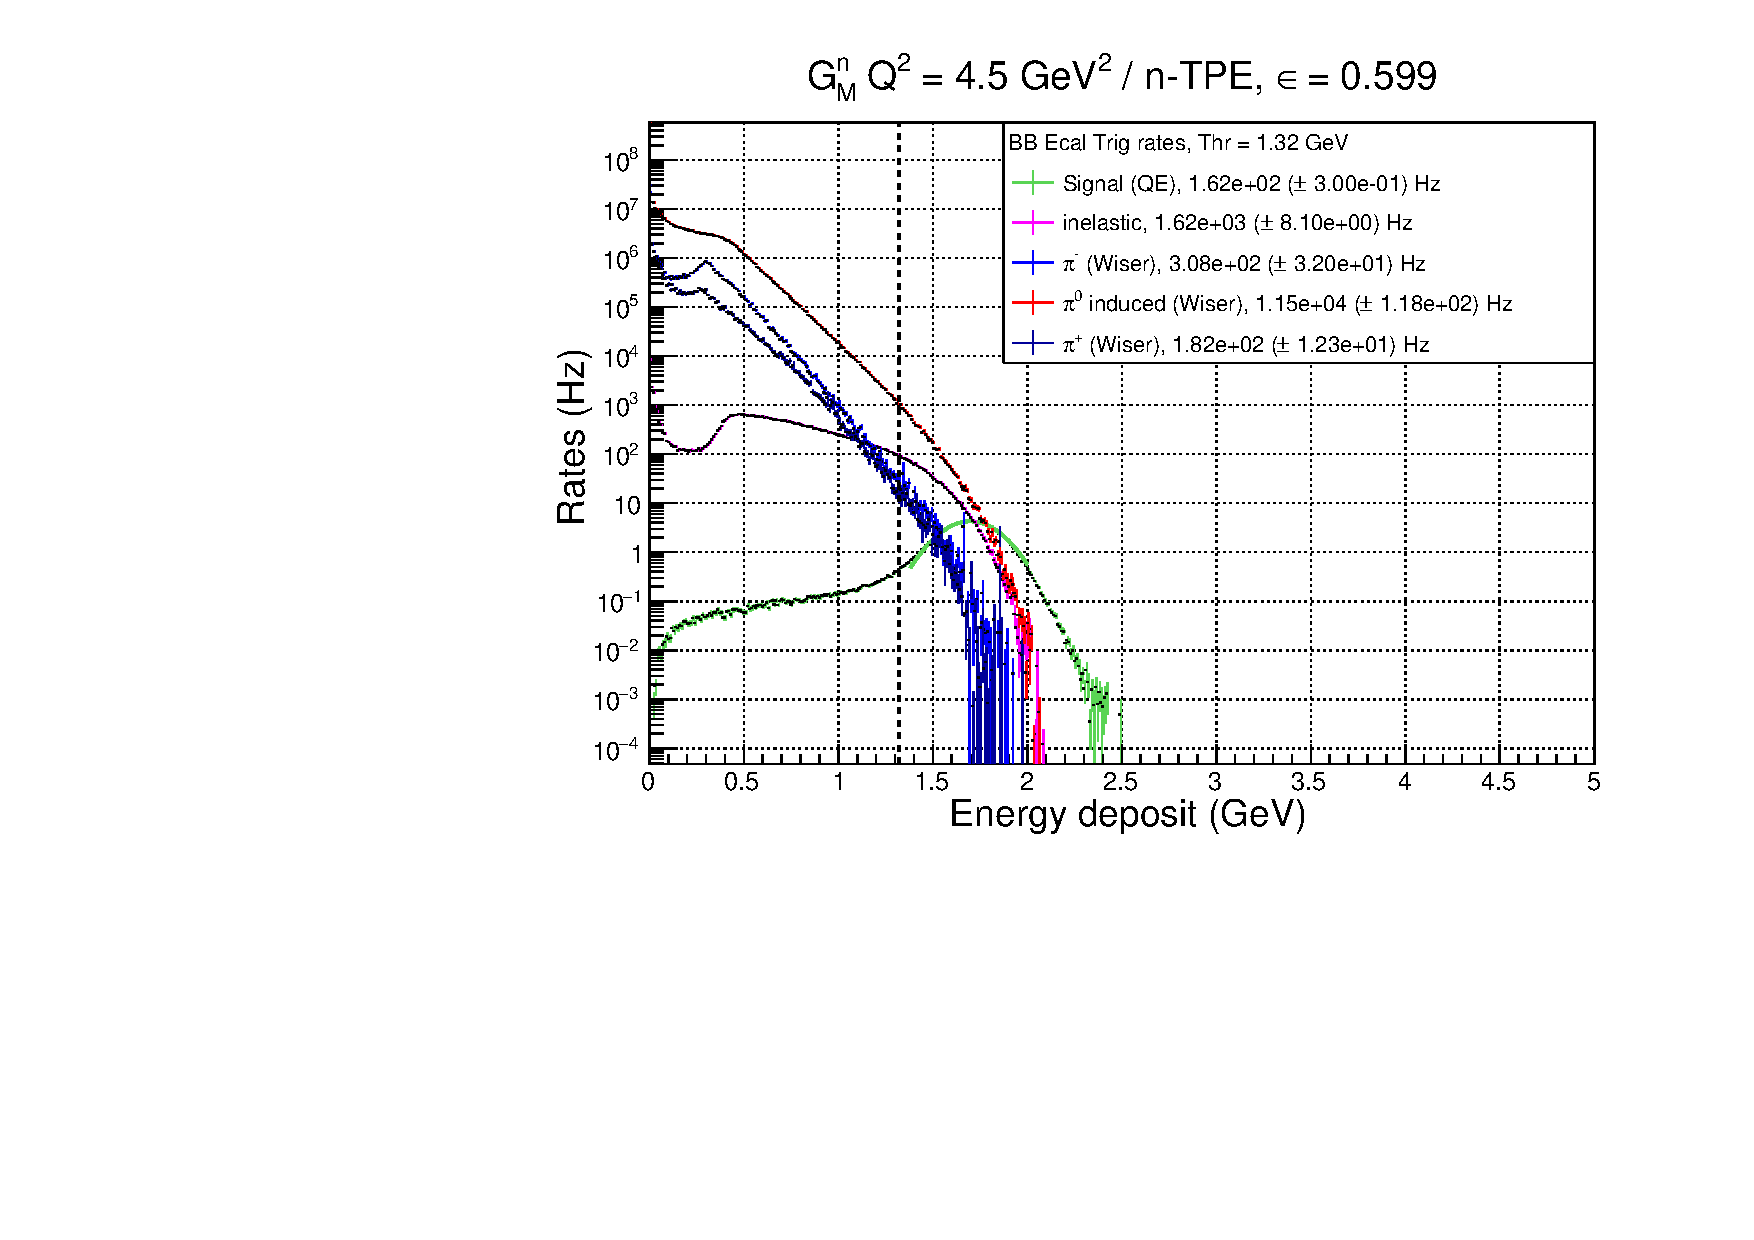
\includegraphics[width=8cm]{Plots/BBECalRates_gen-tpe_le.pdf}
    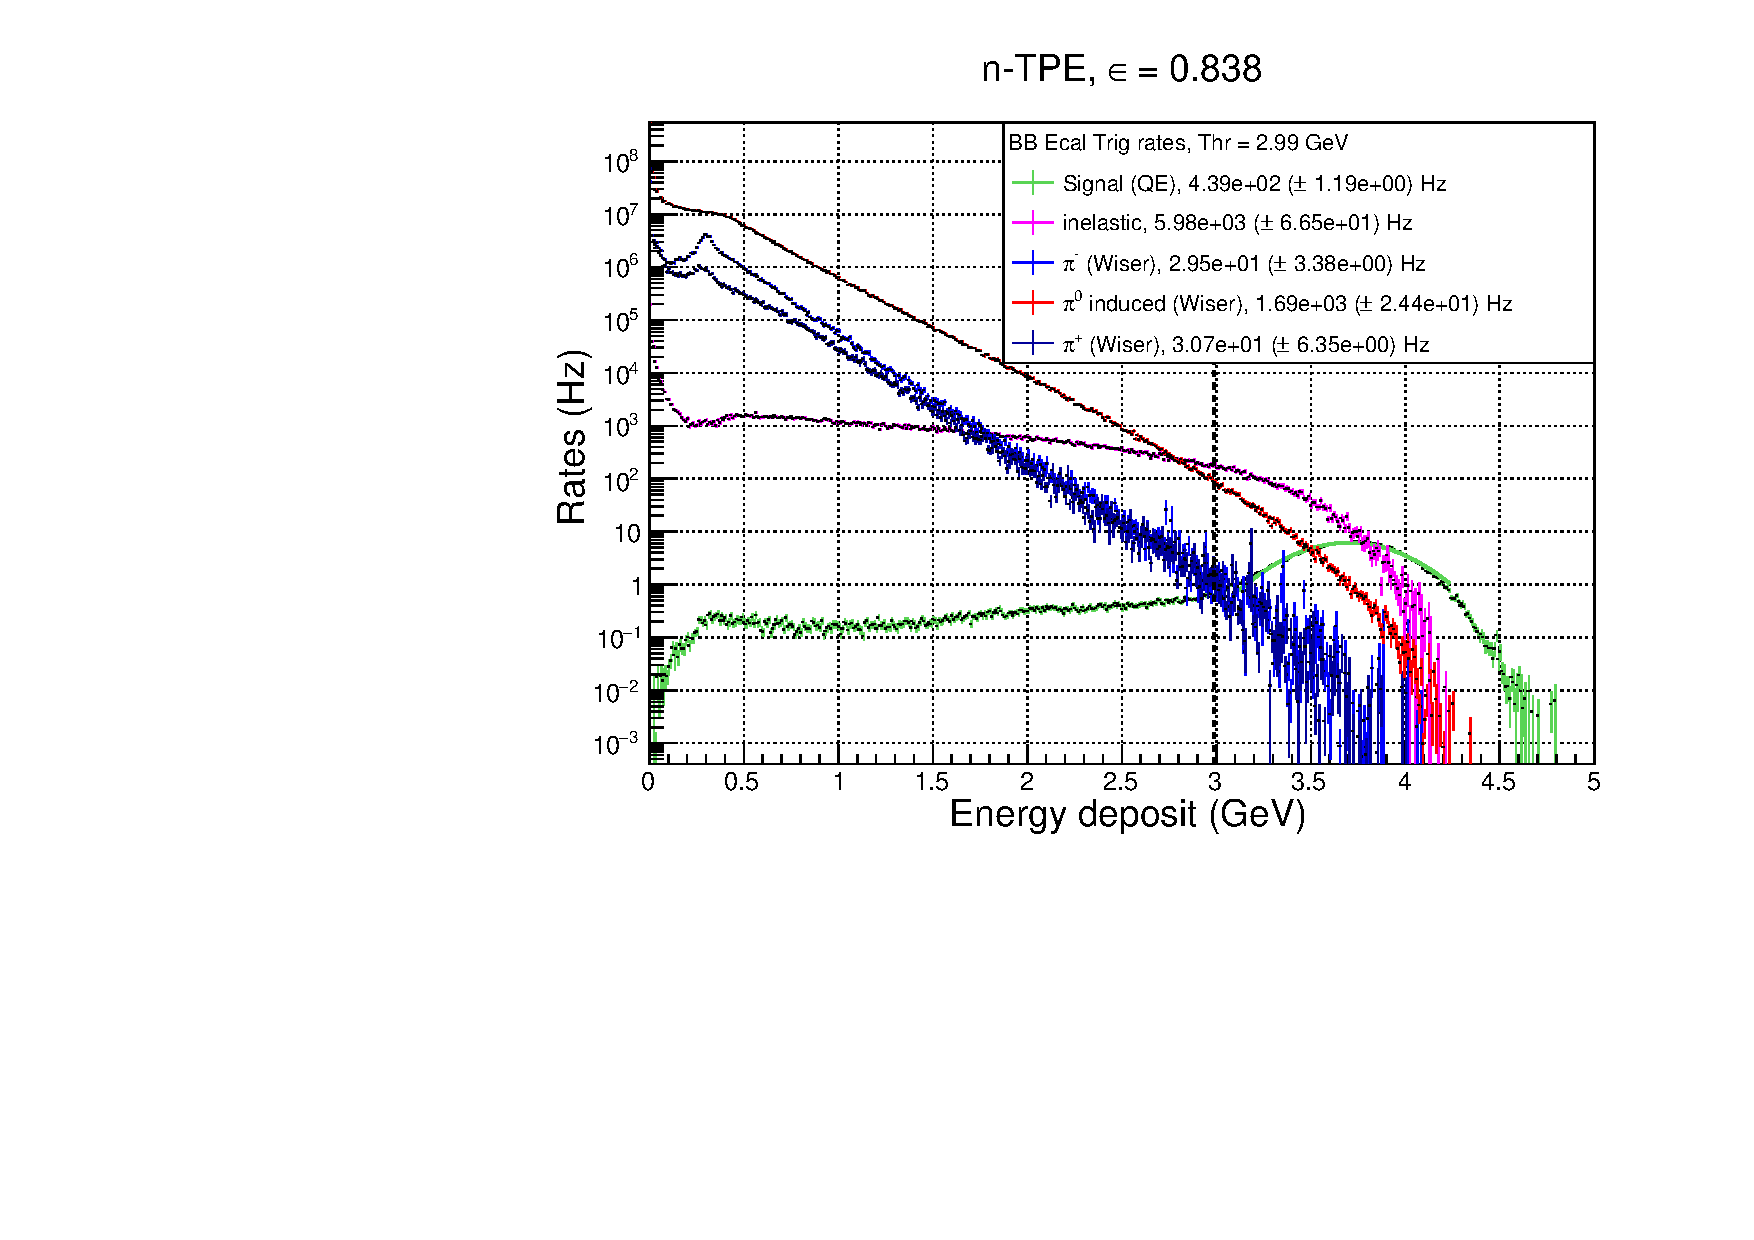
\includegraphics[width=8cm]{Plots/BBECalRates_gen-tpe_he.pdf}
    \caption{Rates of the different process contributing to the BigBite electron arm trigger, for the low $\epsilon$ (left) and the high $\epsilon$ (right). Quasi-elastic is in green, inelastic in magenta, $\pi0$ in red, $\pi^-$ in blue, and $\pi^+$ in dark blue. Note the resolution for the elastic peak in the BigBite shower is $\sim0.3$ GeV.}
    \label{fig:BBRates}
\end{figure}

Since HCal is a sampling calorimeter (meaning that only a fraction of the shower energy is measured), its resolution is relatively wide ($\sim0.7$ GeV).
Due to this, the threshold is at 90\% efficiency (which corresponds to $\sim$0.1 GeV for both kinematics.
Fig.~\ref{fig:HCalRates} presents the distributions of rate of energy deposit for the different processes involved in the HCal trigger rates.
\begin{figure}[h]
  \centering
    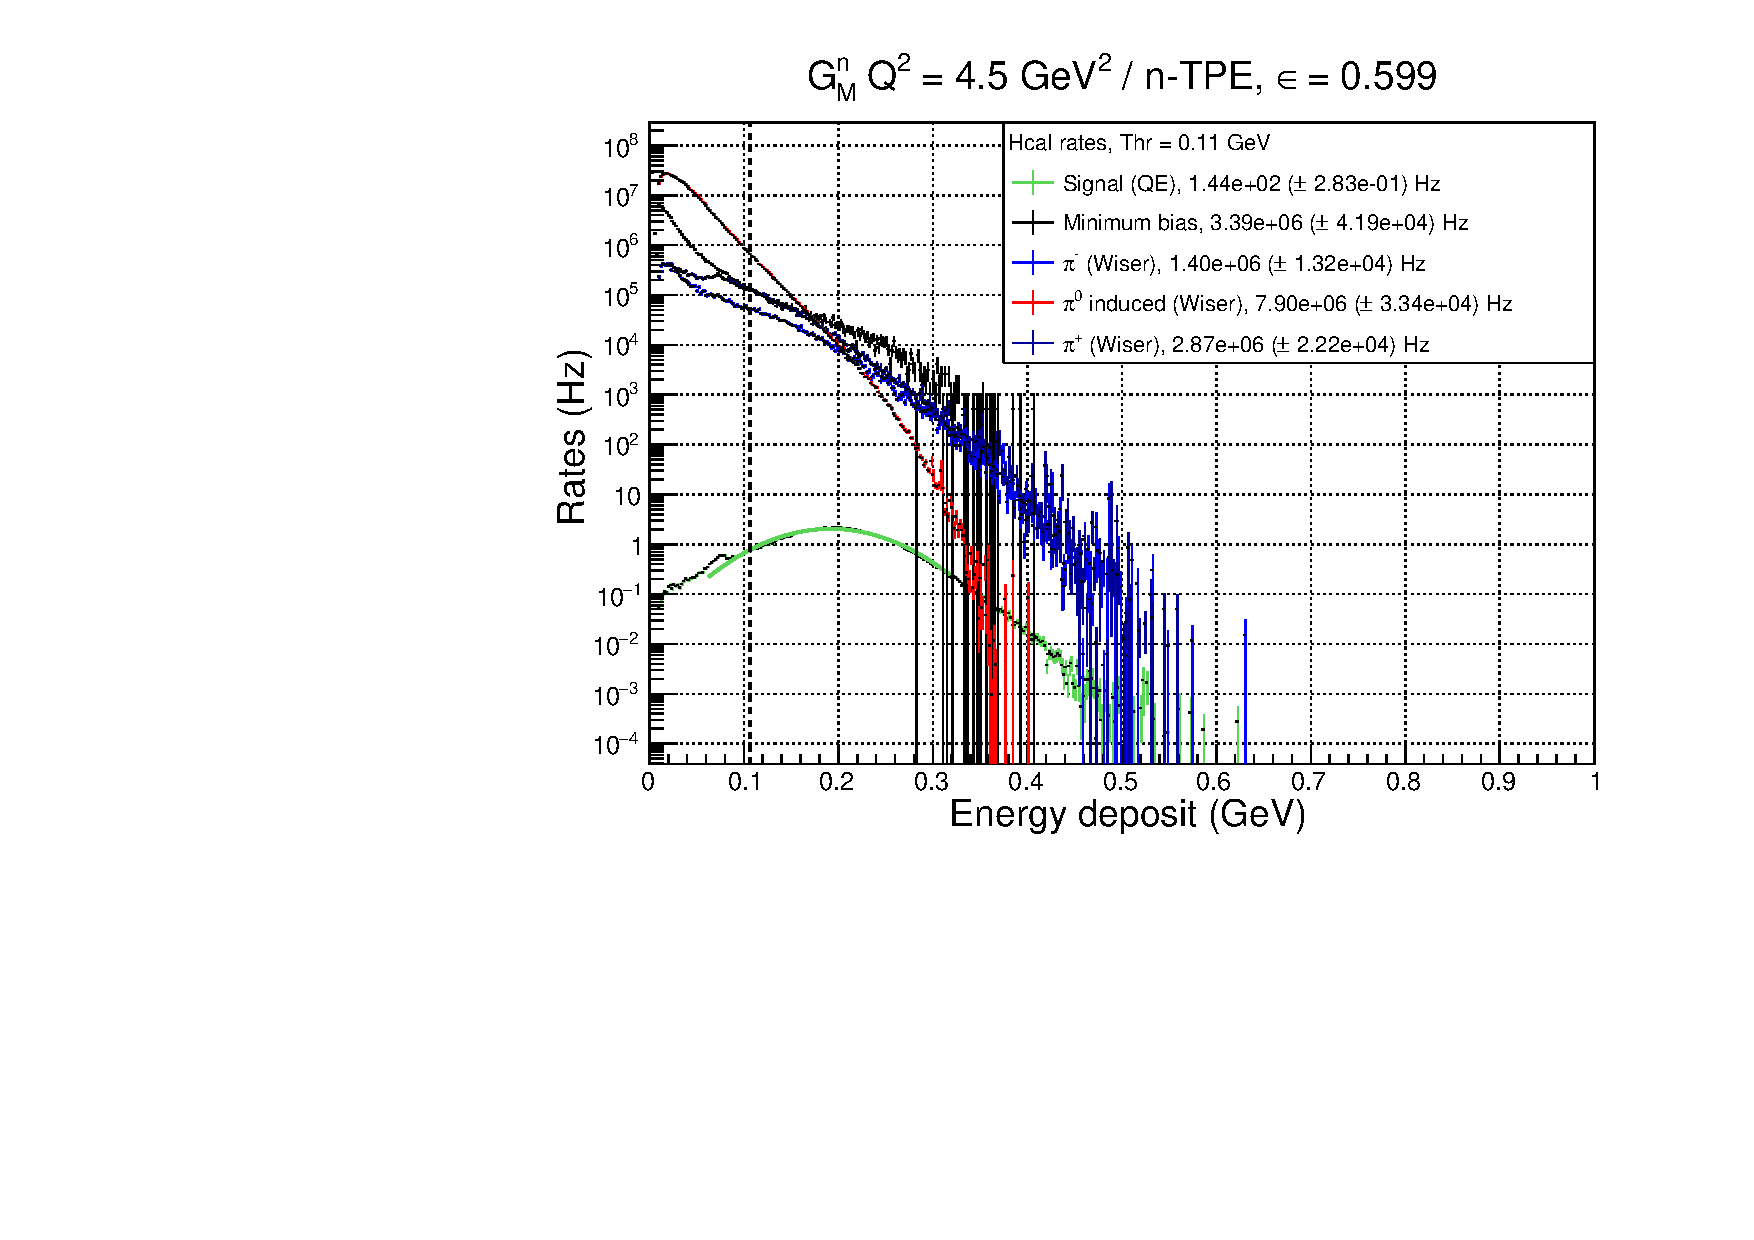
\includegraphics[width=8cm]{Plots/HCalRates_gen-tpe_le.pdf}
    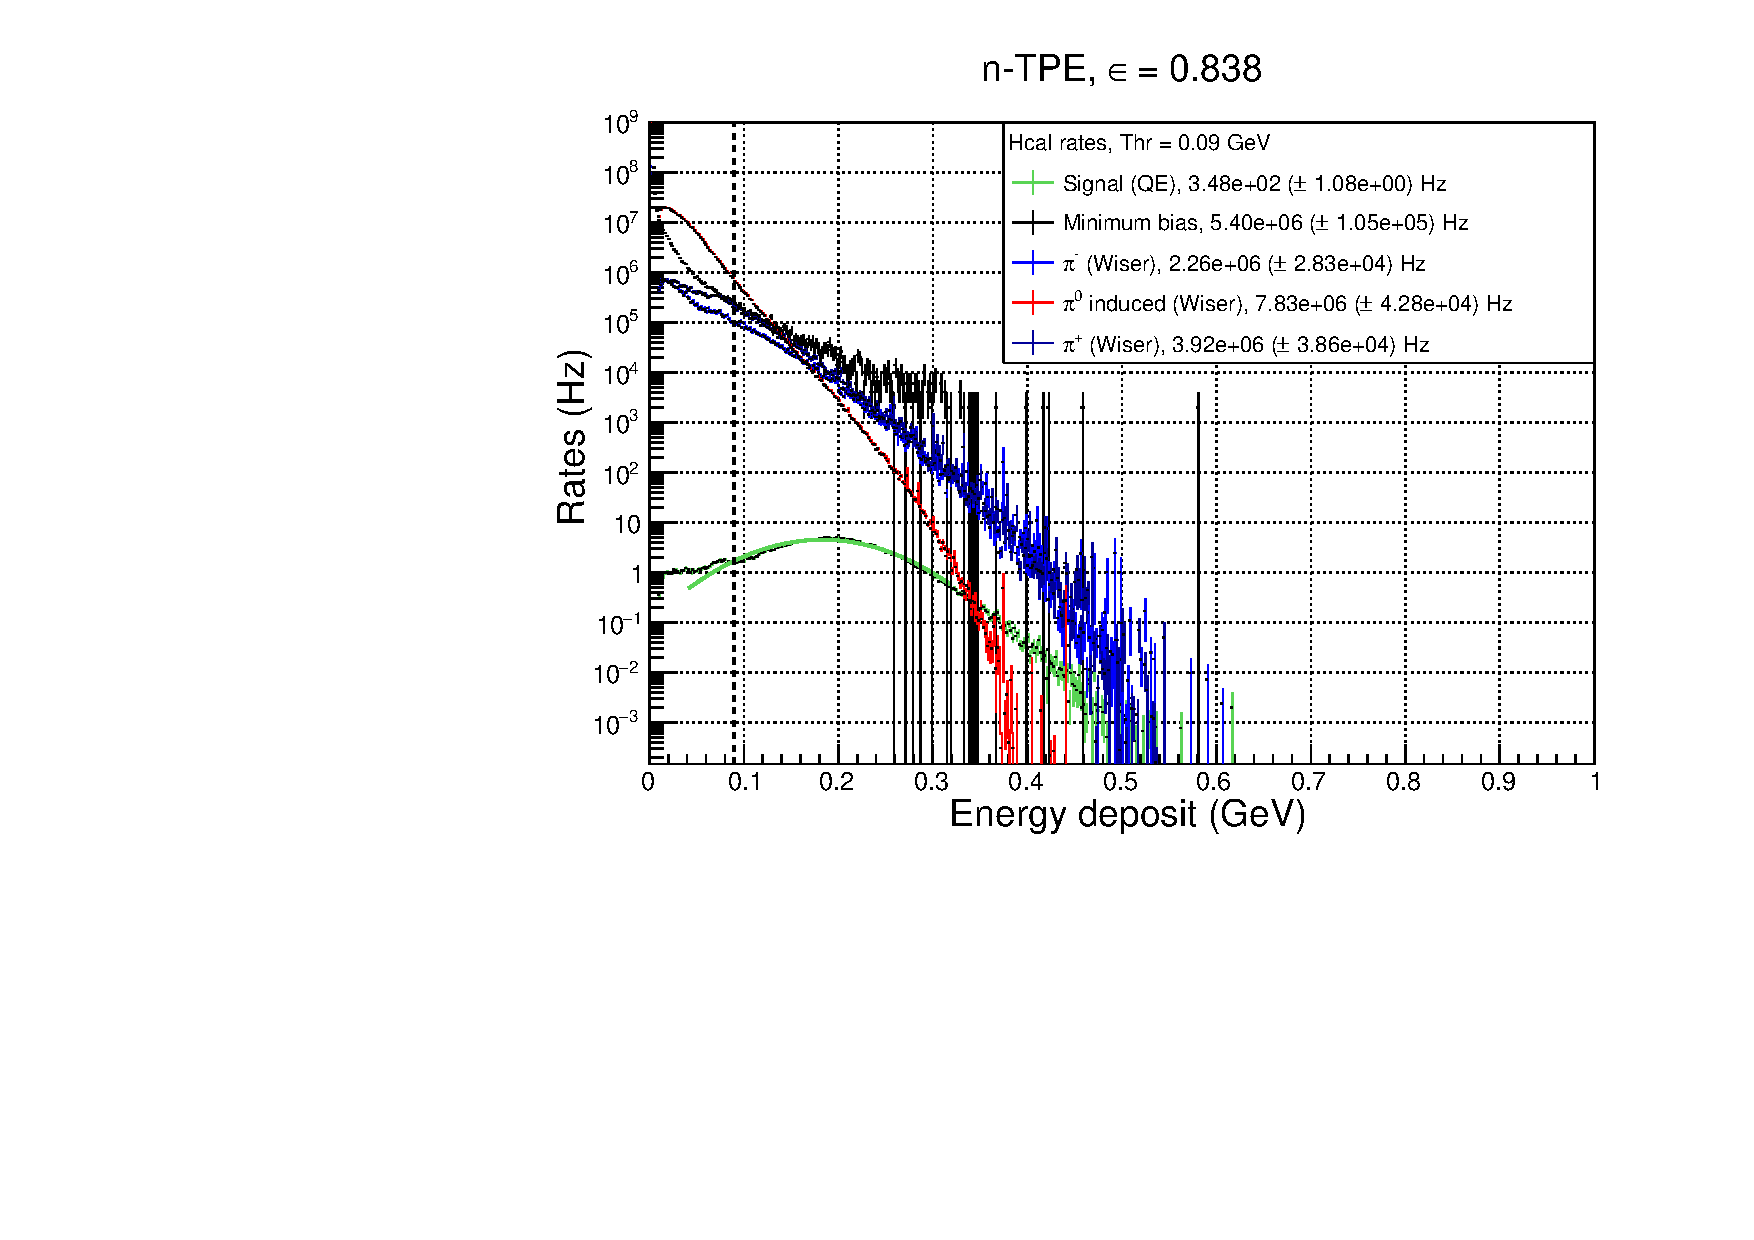
\includegraphics[width=8cm]{Plots/HCalRates_gen-tpe_he.pdf}
    \caption{Rates of the different process contributing to the HCal trigger, for the low $\epsilon$ (left) and the high $\epsilon$ (right). Quasi-elastic is in green, minimum bias in black, $\pi0$ in red, $\pi^-$ in blue, and $\pi^+$ in dark blue. Note the peak itself is around 0.2 GeV for 3.2 GeV nucleons.}
    \label{fig:HCalRates}
\end{figure}

The thresholds and trigger rates for each arm, as well as the coincidence rate (assuming 30ns coincidence window), are summarized in Table.~\ref{tab:TrigRates}.
\begin{table}[h]
\centering
\begin{tabular}{|l|c|c|c|c|}
\hline
Point ($\epsilon$) & \multicolumn{2}{|c|}{1 (0.599)} & \multicolumn{2}{c|}{2 (0.838)} \\
\hline
& BigBite & HCal & BigBite & HCal \\ 
& rates (Hz) & rates (Hz) & rates (Hz) & rates (Hz) \\
\hline
threshold (GeV) & 1.32 & 0.106 & 2.99 & 0.090 \\
\hline
Quasi-elastic   & 1.62$\times 10^{2}$ & 1.44$\times 10^{2}$ & 4.39$\times 10^{2}$ & 3.48$\times 10^{2}$ \\
Inelastic       & 1.62$\times 10^{3}$ & - & 5.98$\times 10^{3}$ & - \\
$\pi^-$ (Wiser) & 3.08$\times 10^{2}$ & 1.40$\times 10^{6}$ & 2.95$\times 10^{2}$ & 1.96$\times 10^{6}$ \\
$\pi^0$ (Wiser) & 1.15$\times 10^{4}$ & 7.90$\times 10^{6}$ & 1.69$\times 10^{3}$ & 5.77$\times 10^{6}$ \\
$\pi^+$ (Wiser) & 1.82$\times 10^{2}$ & 2.87$\times 10^{6}$ & 3.07$\times 10^{2}$ & 3.34$\times 10^{6}$ \\
Minimum bias    & - & 3.39$\times 10^{6}$ & - & 3.32$\times 10^{6}$($^*$) \\ 
\hline
{\em Total} & 1.37$\times 10^{4}$ & 3.39$\times 10^{6}$ & 8.17 $\times 10^{3}$ & 3.32$\times 10^{6}$ \\
($\sum_{\pi (Wiser)}$ for HCal) &  & / (1.22$\times 10^{7}$)  &  & / (1.11$\times 10^{7}$) \\
\hline
{\bf Coincidence rate} & \multicolumn{2}{|c|}{1.39$\times 10^{3}$} & \multicolumn{2}{|c|}{8.14$\times 10^{2}$} \\
($\sum_{\pi (Wiser)}$ for HCal) & \multicolumn{2}{|c|}{(5.01$\times 10^{3}$)} & \multicolumn{2}{c|}{(2.72$\times 10^{3}$)} \\
\hline
\end{tabular} 
\caption{Trigger rates for BigBite and HCal, with the different process contributions separated, and the sum. For HCal, the total rates is either estimated with the minimum bias generator or the sum of inclusive pions estimated with the Wiser cross section. The coincidence rates assume a 30 ns coincidence window.}
\label{tab:TrigRates}
\end{table}
Note that for HCal, the ``total rates'' is either the ``minimum bias'' beam on target, {\em or} the sum of inclusive charged and neutral pions evaluated with the Wiser cross sections. Comparisons between Wiser and minimum bias at very low energy shows that the Wiser code results dramatically overestimate the HCal rates, henceforth the HCal rates estimations using minimum bias are deemed more reliable (and emphasized in Table.~\ref{tab:TrigRates}). For the sake of thoroughness, we have checked the coincidence rates assuming the sum of the inclusive pions (evaluated with the Wiser cross sections) as the HCal rates.

{\em Assuming this worst case scenario}, the coincidence rates could be as high as 5kHz, which might be at the limit of manageability for the DAQ.
However, even if those rates were proven to be accurate, a slight increase on the HCal threshold (which would drop the efficiency from $\sim$90\% to $\sim$85\%) would decrease the total HCal rates by $\sim$35\% to 40\% in this worst case scenario, which would make the situation more manageable (3.3 kHz).
In the more reasonable case where the HCal rates are more accurately described by the minimum bias prediction, the coincidence will be lower than 2kHz, rate at which the SBS DAQ should operate safely.
  
  
\subsection{Contamination from inelastic}\label{sec:inel_contam}
The main source of contamination for the quasi-elastic comes from the inelastic electron-nucleon scattering. Most of this contamination can be cleaned out thanks to a selection on the center of mass energy
%
\begin{equation}
  W^2 = M_{N}^2+2M_{N}^{2}(E-E')-Q^2, %= (q+p)^2 
\end{equation}
%
and the missing transverse momentum of the nucleon
%
\begin{equation}
  p_{\perp miss} = \sqrt{(q_{x}-p'_{x})^2+(q_{y}-p'_{y})^2},
\end{equation}
%
where $M_N$ is the mass of the nucleon, $E$ and $E'$ the initial and final energy of the electron, and $q_{x,y}$, $p'_{x, y}$ are the projections on $x$, $y$ of the vectors of the virtual photon and final nucleon.
The distributions of these quantities (weighted with cross section and including detector resolutions) are displayed for quasi-elastic and inelastic scattering, and for proton and nucleon, on Fig.~\ref{fig:inel_contam_le} for the low $\epsilon$ kinematic, and on Fig.~\ref{fig:inel_contam_he} for the high $\epsilon$ kinematic.\par
\begin{figure}[h]
  \centering
    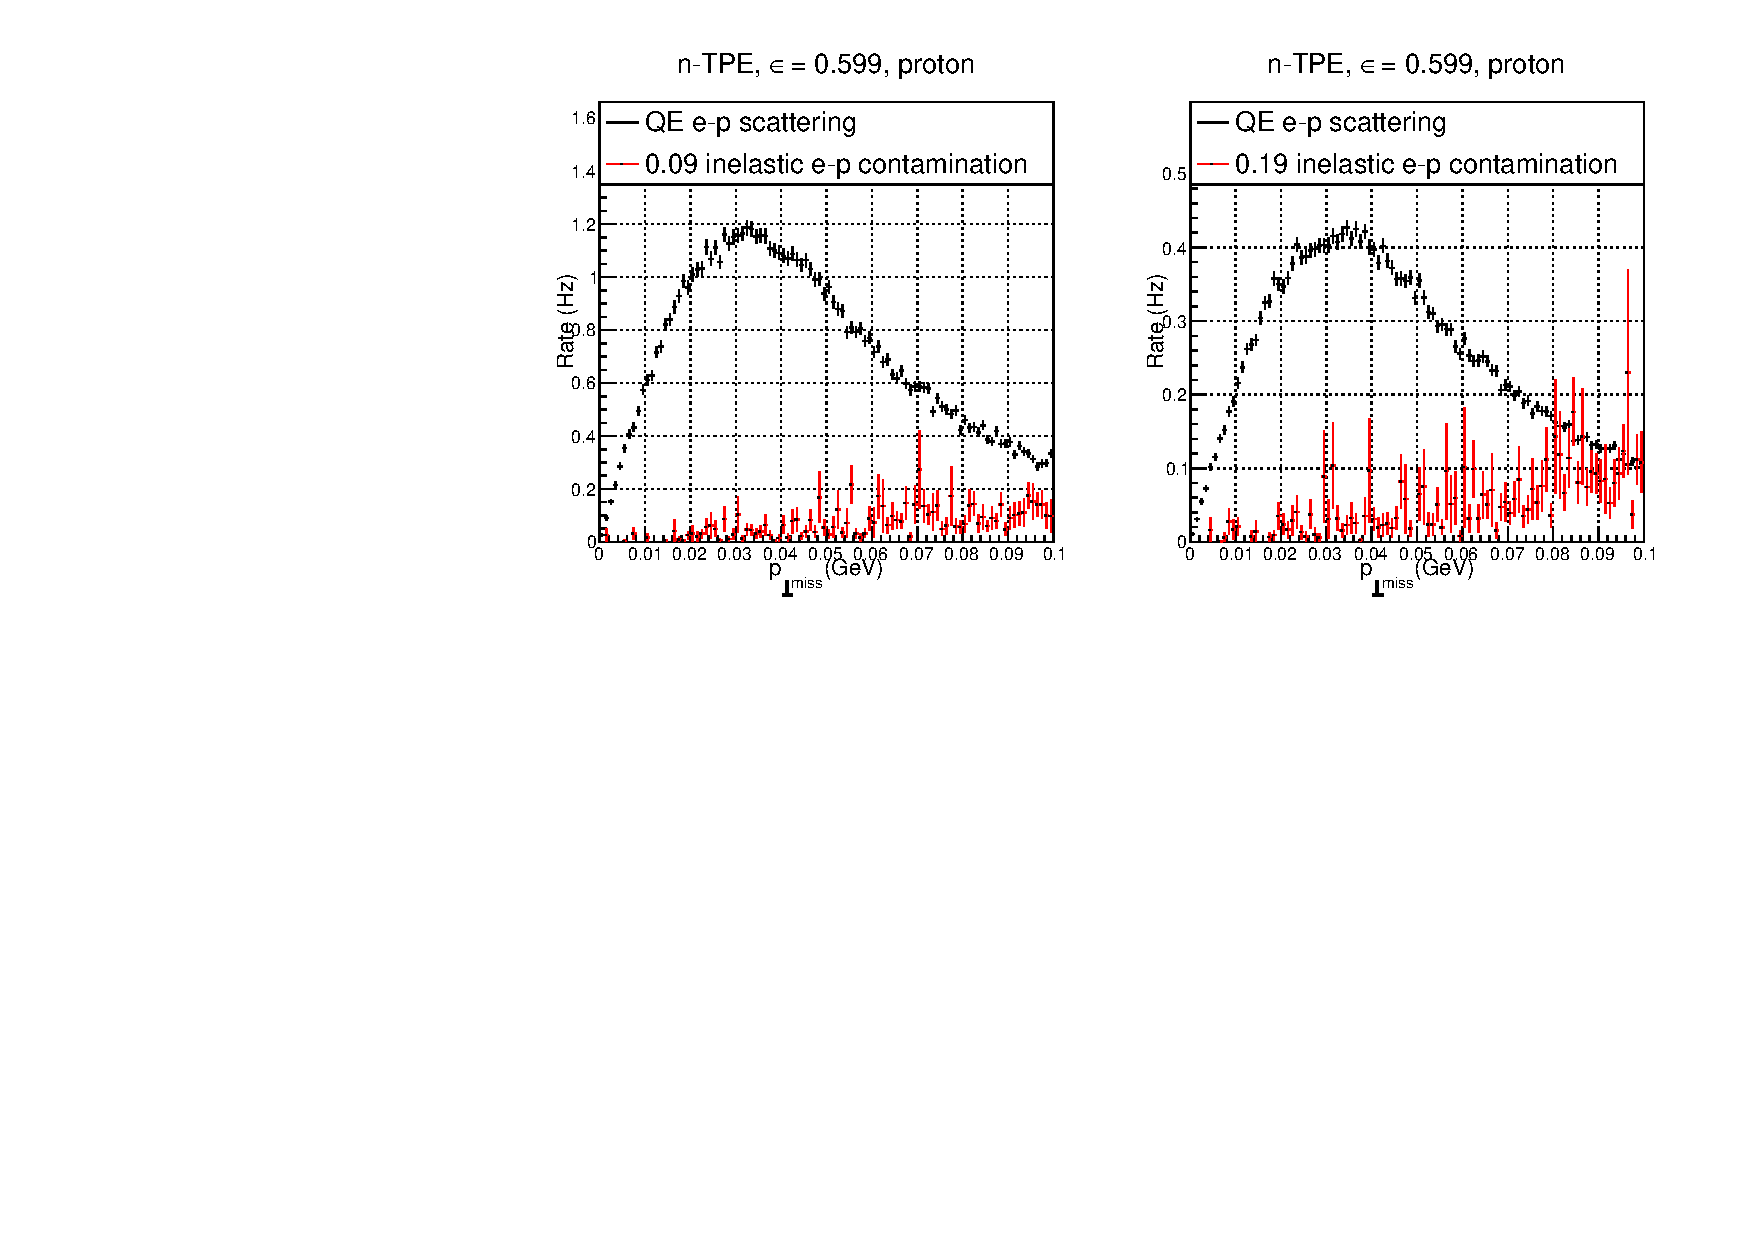
\includegraphics[width=12cm]{Plots/gen-tpe_le_pperp_acc.pdf}
    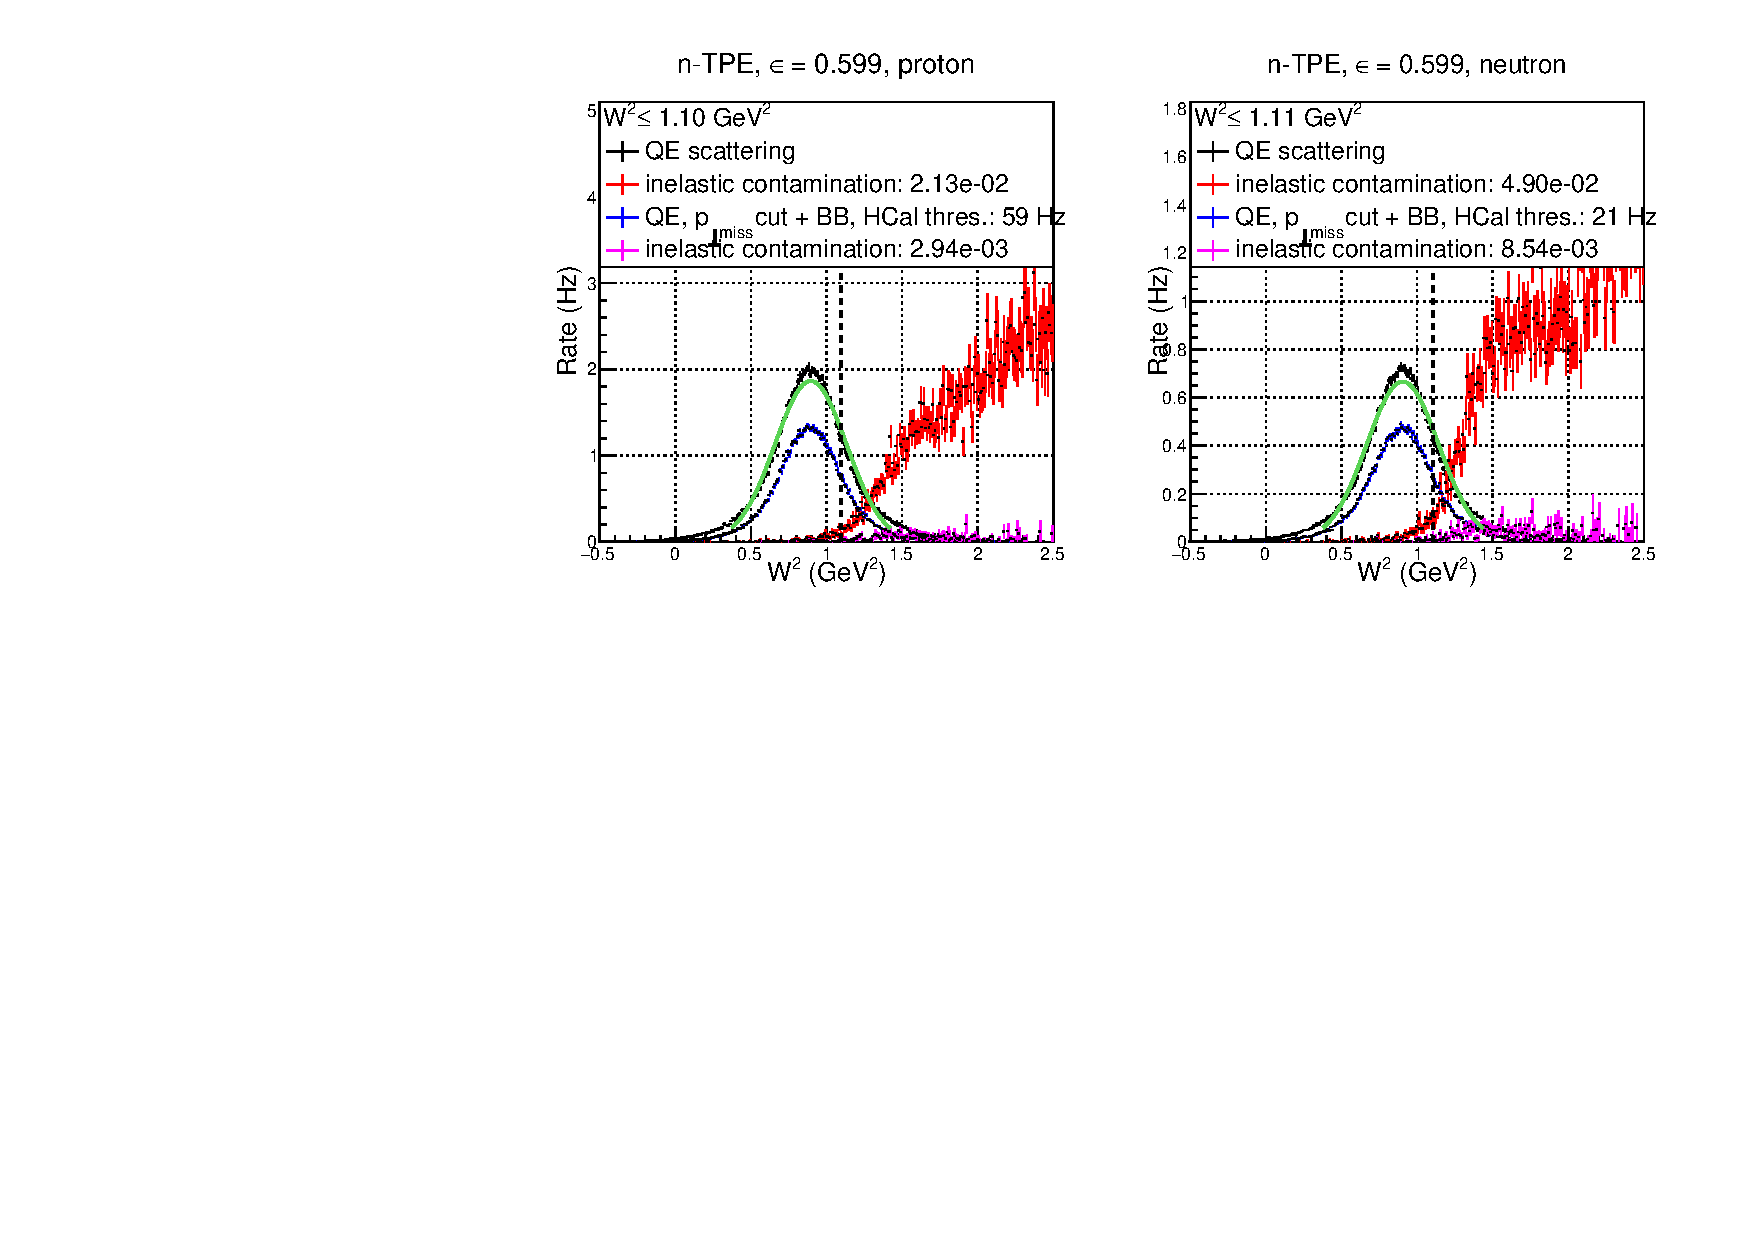
\includegraphics[width=12cm]{Plots/gen-tpe_le_W2_acc.pdf}
    \caption{Compared quasi-elastic and inelastic distributions (including detectors resolutions) for $p_{\perp miss}$ (top) and $W^2$ (bottom), for the low $\epsilon$ kinematic. Comparison for protons is on the left, and comparison for neutrons is on the right. On the bottom panel, black and red are before the $p_{\perp miss}~\leq~0.1~\mathrm{GeV}$ selection, while blue and magenta are after $p_{\perp miss}~\leq~0.1~\mathrm{GeV}$ selection and application of BigBite shower and HCal thresholds.}
    \label{fig:inel_contam_le}
\end{figure}
\begin{figure}[h]
  \centering
    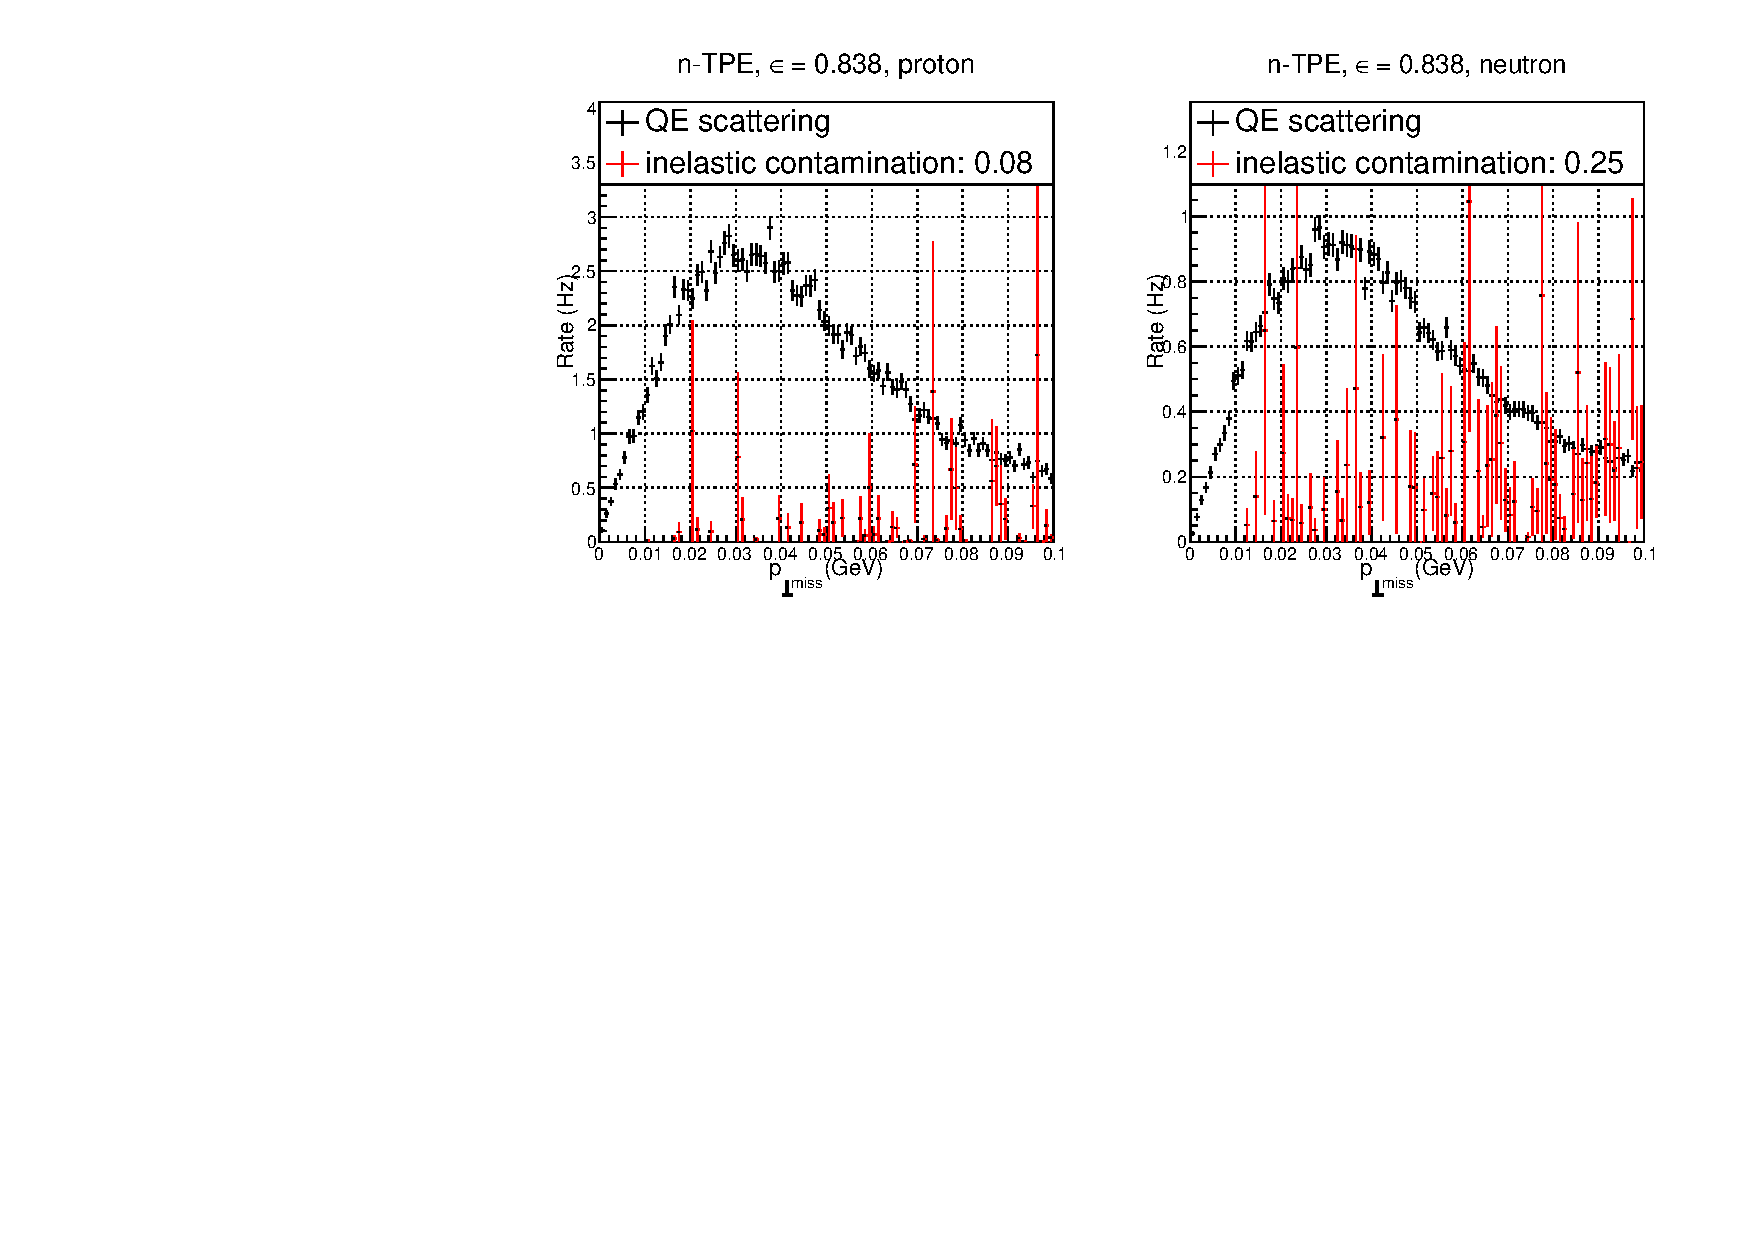
\includegraphics[width=12cm]{Plots/gen-tpe_he_pperp_acc.pdf}
    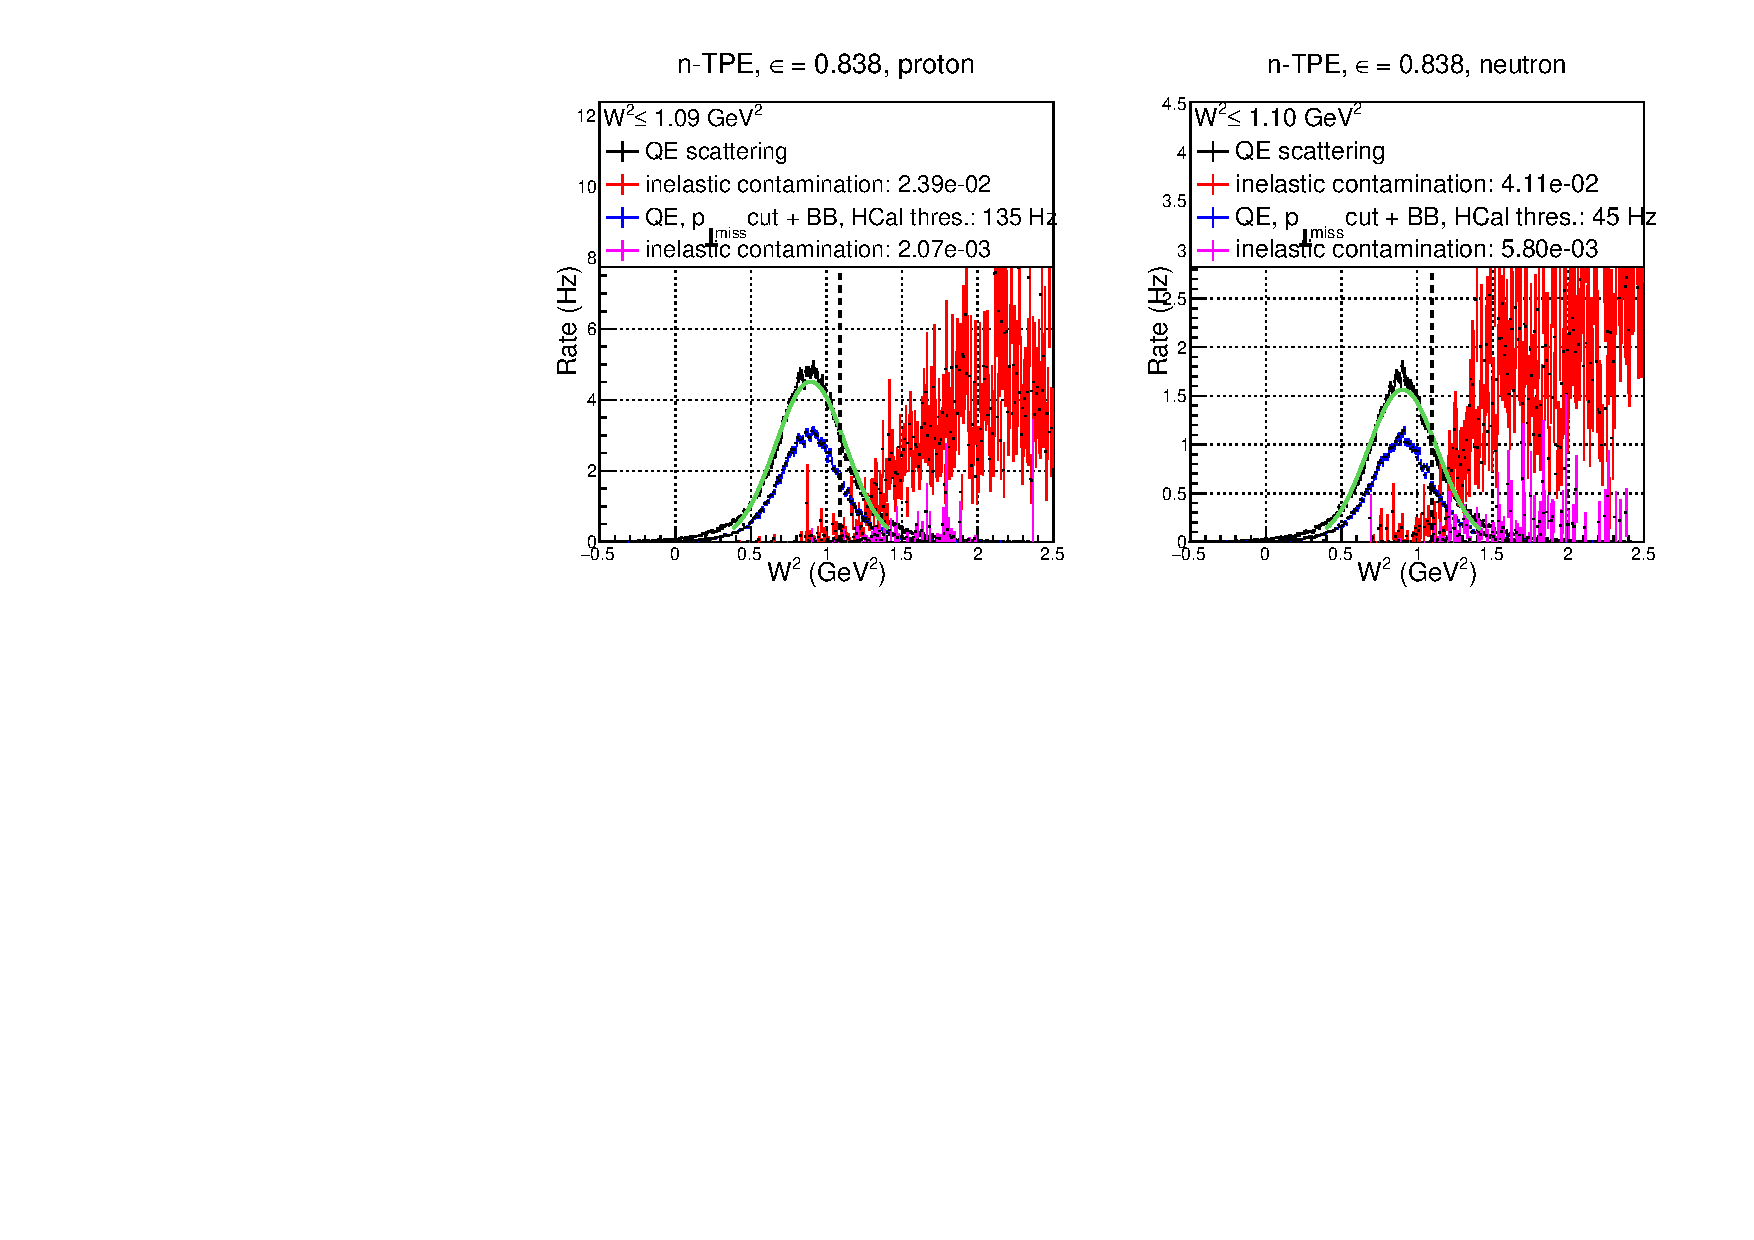
\includegraphics[width=12cm]{Plots/gen-tpe_he_W2_acc.pdf}
    \caption{Compared quasi-elastic and inelastic distributions (including detectors resolutions) for $p_{\perp miss}$ (top) and $W^2$ (bottom), for the high $\epsilon$ kinematic. Comparison for protons is on the left, and comparison for neutrons is on the right. On the bottom panel, black and red are before the $p_{\perp miss}~\leq~0.1~\mathrm{GeV}$ selection, while blue and magenta are after $p_{\perp miss}~\leq~0.1~\mathrm{GeV}$ selection and application of BigBite shower and HCal thresholds.}
    \label{fig:inel_contam_he}
\end{figure}

Provided that we are not limited by statistics and we prioritize sample purity is capital for our experiment, we set the selection criteria on $W^2$ and $p_{\perp miss}$ to minimize inelastic contamination (ideally below 1~\%). 
Setting $p_{\perp miss}~\leq~0.1~\mathrm{GeV}$ and $W^2~\leq~1.1~\mathrm{GeV}^2$, the inelastic contamination of the elastic sample ranges from 0.2~\% to 0.9~\%, while retaining $\geq$~60~\% of the quasi-elastic events properly recorded in the BigBite-SBS pair.
Table.~\ref{tab:contam} summarizes the quasi-elastic selection cuts, and inelastic contamination $\delta_{inel}$.

\begin{table}[h]
\centering
\begin{tabular}{|c|c|c|c|c|}
\hline
Point ($\epsilon$) & $N$ & $W^2$ cut & $p_{\perp miss}$ cut & $\delta_{inel}$ \\
\hline
1 (0.599) & $n$ & 1.10 & 0.10 & 2.94~$\times 10^{-3}$ \\
 & $p$ & 1.11 & 0.10 & 8.54~$\times 10^{-3}$ \\
\hline
2 (0.838) & $n$ & 1.09 & 0.10 & 2.07~$\times 10^{-3}$ \\
 & $p$ & 1.10 & 0.10 & 5.80~$\times 10^{-3}$ \\
\hline
\end{tabular} 
\caption{Summary of cuts for quasi-elastic selection and resulting inelastic contamination $\delta_{inel}$.}
\label{tab:contam}
\end{table}

\subsection{Quasi-elastic counting rates}

The signals for this experiment have been generated using the G4SBS elastic/quasi-elastic generator. 
We generated a reasonably large sample of quasi-elastic events $N_{Gen}$ for each kinematics, within a solid angle $\Delta\Omega_{Gen}$ that was larger than the detector acceptance.
To evaluate the detector solid angle, we define simple criteria that each event has to pass, defined as follows:
%
\begin{itemize}
\item{require a primary track, going through all 5 GEM layers (electron arm);}
\item{require non-zero energy deposit in both the preshower and shower (electron arm);}
\item{require non-zero energy deposit in HCal (hadron arm).}
\end{itemize}
%
The detector solid angle, for both proton and neutron, are defined in Table.~\ref{tab:kinExpParams}.
We also define there the $p$-$n$ acceptance asymmetry $A_{\Delta\Omega}$ such as:
\begin{equation}
  A_{\Delta\Omega} = \frac{(\Delta\Omega_e \otimes \Delta\Omega_n)-(\Delta\Omega_e \otimes \Delta\Omega_p)}{(\Delta\Omega_e \otimes \Delta\Omega_n)+(\Delta\Omega_e \otimes \Delta\Omega_p)}
\end{equation}

\begin{table}[h]
\centering
\begin{tabular}{|c|c|c|c|c|}
\hline
Point ($\epsilon$) & $\Delta\Omega_e$ & $\Delta\Omega_e \otimes \Delta\Omega_n$ & $\Delta\Omega_e \otimes \Delta\Omega_p$ & $A_{\Delta\Omega}$ \\
 & (msr) & (msr) & (msr) & (\%) \\
\hline
1 (0.599) & 52.4 & 46.7 & 47.2 & 0.5 \\
\hline
2 (0.838) & 32.7 & 20.8 & 22.2 & 3.0 \\
\hline
\end{tabular} 
\caption{Kinematics electron solid angle, and convoluted electron/hadron solid angle, and acceptance asymmetry.}
\label{tab:kinExpParams}
\end{table}

Then, we evaluate the detection efficiency. For the electron, we require the energy reconstructed in the BigBite calorimeter to be above a threshold defined as $thr = \mu_E- 2.5* \sigma_E$, as well as a minimum number of GRINCH PMTs fired due to the primary electron; For HCal, we select a threshold that yields~90\%~efficiency. These values are summarized in Table.~\ref{tab:kinEffs}.
Quasi-elastic selection efficiency $\eta_{sel}$ are also provided.

\begin{table}[h]
\centering
\begin{tabular}{|c|c|c|c|c|c|c|c|}
\hline
Point ($\epsilon$) & BB thr. & HCal thr. & $\eta_{det~e}$ & $\eta_{det~n}$ & $\eta_{det~p}$ & $\eta_{sel~n}$ & $\eta_{sel~p}$ \\
 & (GeV) & (GeV) &  &  &  &  &  \\
\hline
1 (0.599) & 1.32 & 0.11 & 0.902 & 0.904 & 0.892 & 0.589 & 0.605 \\ 
\hline
2 (0.838) & 2.99 & 0.09 & 0.808 & 0.889 & 0.882 & 0.617 & 0.647 \\
\hline
\end{tabular} 
\caption{Kinematics electron thresholds, particle detection efficiencies ($\eta_{det}$), and efficiency of quasi-elastic selection $\eta_{sel}$ separated for the proton and the neutron.}
\label{tab:kinEffs}
\end{table}
The counting rates are evaluated using among the $N_{Gen}$ events generated the events that have passed the selection described below, and weighting those events with the cross section ${d\sigma}/{d\Omega}|_i$ calculated by G4SBS, multiplied by the generation solid angle $\Delta\Omega_{Gen}$, using the formula:
\begin{equation}
  N_{est} = \frac{{\cal L}_{exp} \Delta t}{N_{Gen}} \times \sum_{i \in accepted~evts}\left( \left. \frac{d\sigma}{d\Omega}\right|_i \times \Delta\Omega_{Gen} \right) \;,
\end{equation}
where $\Delta t$ the running time and ${\cal L}_{exp}$ the experimental luminosity. ${\cal L}_{exp}$ can be calculated as follows:
\begin{equation}
  {\cal{L}}_{exp} = \frac{I_{exp}}{q_e}\cdot L_{tgt}\cdot d_{tgt}\;\frac{\cal{N}_A}{m_{D}}\;,
\end{equation}
where $I_{exp}$ is the beam current, $q_e$ is the electron charge, $L_{tgt}$ and $d_{tgt}$ are the target length and density respectively, $N_A$ is Avogadro's number, and $m_D$ is the deuterium mass number.
Events are ``accepted'' if they meet the following criteria:
%
\begin{itemize}
\item{the electron is in the BigBite acceptance};
\item{the electron passes the BigBite threshold defined in Table~\ref{tab:kinEffs} and gives signal in the GRINCH;}
\item{the nucleon is in the HCal acceptance and passes the HCal threshold defined in Table~\ref{tab:kinEffs};}
\item{the event passes the quasi-elastic selection defined in the previous section {\it i.e.} $W^2~\leq~1.1~\mathrm{GeV}^2$ and $p_{\perp miss}~\leq~0.10~\mathrm{GeV}$.} 
\end{itemize}
%

The total quasi-elastic statistics $N_{QE}$, as well as the total form factor, $F^2$:
\begin{equation}
  F^2 = \frac{N_{QE}}{{\cal{L}}_{exp} \cdot \Delta t \cdot  d\sigma_{Mott}/d\Omega  \cdot \Delta\Omega \cdot  \eta}
  \label{eq:F2}
\end{equation}
and its statistical error $\Delta F^2 = F^2/\sqrt{N_{QE}}$ are compiled for both kinematics in Table.~VI%\ref{tab:Rates}
, assuming a running time $\Delta t = 12$~hours of running at a beam intensity of $I_{exp} =~30~\mu$A on a liquid deuterium target with length $l_{tgt}~=~15$~cm and density $d_{tgt}~=~0.169~\mathrm{g.cm}^{-3}$. In Eq.~13%\ref{eq:F2}
, $\Delta\Omega$ is the convoluted BigBite-HCal solid angle, and $\eta$ is the product of all efficiencies (detection efficiencies $\eta_{det}$ $\times$ selection efficiency $\eta_{sel}$). 

\begin{table}[h]
\centering
\begin{tabular}{|c|c|c|c|c|c|c|}
\hline
Point ($\epsilon$) & $N_{QE}$ & $N_{QE}$ & $F^2_n$ & $\Delta F^2_n$ & $F^2_p$ & $\Delta F^2_p$ \\
 &  ($e$-$n$) &  ($e$-$p$) & ($\times 10^{-3}$) & ($\times 10^{-6}$) & ($\times 10^{-3}$) & ($\times 10^{-6}$) \\
\hline
1 (0.599) & 9.07$\times 10^{5}$ & 2.55$\times 10^{6}$ & 0.99 & 1.04 & 2.73 & 1.70 \\
\hline
2 (0.838) & 1.94$\times 10^{6}$ & 5.83$\times 10^{6}$ & 0.72 & 0.52 & 1.93 & 0.80 \\
\hline
\end{tabular} 
\caption{Quasi-elastic counting rates, and total form factor (defined in Eq.~11).}%({\em preliminary})
\label{tab:Rates}
\end{table}

The calculation of the $F_2$ term requires the evaluation of the Mott cross section:
%
\begin{equation}
  \sigma_{Mott} \equiv  \frac{d\sigma_{Mott}}{d\Omega} = (\hbar c\alpha_{EM})^2
  \frac{1}{4E^2} \left( \frac{\cos{\theta_e/2}}{\sin^2{\theta_e/2}} \right)^2 \frac{E'}{E}
\end{equation}
%
%\textcolor{red}{{\it private note}: $\hbar c$ is in $\mathrm{GeV}\cdot\mathrm{cm}^{-1}$, but I've assumed $e=1$.}\\
The Mott cross section has been calculated with the weighted average of the electron variables (momentum and polar angle).

\begin{table}[h]
\centering
\begin{tabular}{|c|c|c|c|c|}
\hline
Point ($\epsilon$) & $\langle \theta_e \rangle$ &  $\langle k^{\prime} \rangle$ & $\langle Q^2 \rangle$ & $\sigma_{Mott}$ \\
 & (deg) & (GeV) & (GeV$^2$) & (nb sr$^{-1}$) \\
\hline
1 (0.599) & 41.88 & 2.0 & 4.5 & 6.62 \\ 
\hline
2 (0.838) & 23.23 & 4.2 & 4.5 & 44.2 \\
\hline
\end{tabular} 
\caption{The Mott cross section weighted average of kinematic variables over the BigBite acceptance.}
\label{tab:sigma_mott}
\end{table}
%

\iffalse
The counting rates for the low $\epsilon$ kinematics should be directly comparable to the rates reported in the original $G_M^n$ proposal \cite{gmp}.
In this proposal, the requested running time was 12 hours, with a beam intensity of 10 $\mu$A on a 10 cm long liquid deuterium target with density 0.169~g.cm$^{-3}$.
This luminosity is 4.5 times lower than the currently proposed luminosity.
%
\begin{center}
\begin{table}[h]
\begin{tabular}{|l|c|c|}
\hline
 & $d(e, e'n)p$ & $d(e, e'p)n$ \\
\hline
This estimation & 3.27$\times 10^{4}$ & 9.00$\times 10^{4}$ \\
\hline
Original proposal Table.~8 & 1.20$\times 10^{4}$ & 2.66$\times 10^{4}$ \\ 
\hline
Discrepancy factor & 2.73 & 3.38 \\ 
\hline
\end{tabular} 
\caption{{\em Hourly} rates comparison between these predictions and the original $G_M^n$ proposal, {\em at the original proposal luminosity} (10.5 $\mu$A on a 10cm liquid deuterium target, with density 0.169 g.cm$^{-3}$). There's a factor 3 discrepancy between the numbers}
\label{tab:RateComp}
\end{table}
\end{center}
\fi

